\makeheading{2020-03-06}
\section{Applications of König's Theorem}
The matching problem for bipartite graphs is in Co-NP\@.

Q\@: Given a bipartite graph $ G $ with bipartition $ (A,B) $,
when does $ G $ have a matching saturating $ A $?

If $ |A|=|B| $, then this is asking for a \textbf{\emph{perfect matching}} of $ G $,
which is a matching that saturates every vertex. Note that,
if some vertex in $ A $ has no neighbours in $ B $, there is no matching saturating $ A $.
The same is true if there are two vertices $ u,v $ in $ A $ such that $ u $ and $ v $
both only have one neighbour $ w $ in $ B $.

For each set $ A^\prime \subseteq A $, let $ N(A^\prime) $ denote the set of vertices
$ B $ having a neighbour in $ A^\prime $.

\begin{thmbox}
    \begin{prop}
        If $ A^\prime\subseteq A $ is a set for which $ |N(A^\prime)|<|A^\prime| $,
        then $ G $ has no matching saturating $ A $.
    \end{prop}
\end{thmbox}
\begin{proof}
    A matching saturating $ A $ must matching each vertex in $ A^\prime $ to a distinct
    vertex in $ N(A^\prime) $, but $ N(A^\prime) $ is too small for there to
    exist this many distinct vertices.
\end{proof}
\begin{thmbox}
    \begin{theorem}[Hall's Theorem]
        Let $ G $ be a bipartite graph with bipartition $ (A,B) $. Then exactly one
        of the following holds.
        \begin{enumerate}[label=(\arabic*)]
            \item $ G $ has a matching saturating $ A $
            \item There is a set $ A^\prime \subseteq A $ such that $ |N(A^\prime)|<|A^\prime| $
        \end{enumerate}
        In other words, $ G $ has a matching saturating $ A $ if and only if $ |N(A^\prime)|\geqslant |A^\prime| $
        for all $ A^\prime \subseteq A $.
    \end{theorem}
\end{thmbox}
\begin{proof}
    We have seen that $ (2)\implies (1) $ doesn't hold. $ (2)\implies \lnot (1) $.
    It is now enough to show that $ \lnot(2)\implies (2) $. Suppose that $ (1) $ doesn't hold;
    that is, $ G $ has no matching saturating $ A $. Let $ M $ be a maximum matching of $ G $,
    so $ |M|<|A| $. By König's Theorem, $ G $ has a cover $ C $ of size $ |M|<|A| $.
    Let $ C_A = C\cap A $ and $ C_B = C\cap B $. Let $ A^\prime=A\setminus C_A $. Since
    $ C $ is a cover, we know that $ N(A^\prime)\subseteq C_B $. Now
    \begin{equation*}
        \begin{aligned}
            |N(A^\prime)|
             & \leqslant |C_B|                                          \\
             & \leqslant |C|-|C_A| & \quad & \text{since }C=C_A\cup C_B \\
             & =|M|-|C_A|          &       & \text{by~\ref{konig}}      \\
             & < |A|-|C_A|         &       & \text{by assumption}       \\
             & =|A^\prime|
        \end{aligned}
    \end{equation*}
    so $ (2) $ holds because $ |N(A^\prime)|<|A^\prime| $.
\end{proof}
\begin{remark}
    Assignment 10 can now be completed up to this point.
\end{remark}

\textbf{\underline{Chess}}

\underline{Problem}: Given a square $ n\times n $ array, find a set $ X $
of $ n $ cells in the array, with no two in the same row or column.
Let $ A $ be the set of rows, $ B $ be the set of columns.

\begin{thmbox}
    \begin{prop}
        If there is a set $ A^\prime \subseteq A $ and a set $ B^\prime \subseteq B $
        such that $ |A^\prime|+|B^\prime|>n $ and every cell in $ A^\prime \times B^\prime $
        is `blocked', then placing $ n $ non-attacking rooks is impossible.
    \end{prop}
\end{thmbox}
\begin{proof}
    $ |A^\prime| $ rooks must be placed in $ \leqslant n-|B^\prime|<|A^\prime| $
    different columns.
\end{proof}

\begin{figure}[H]
    \centering
    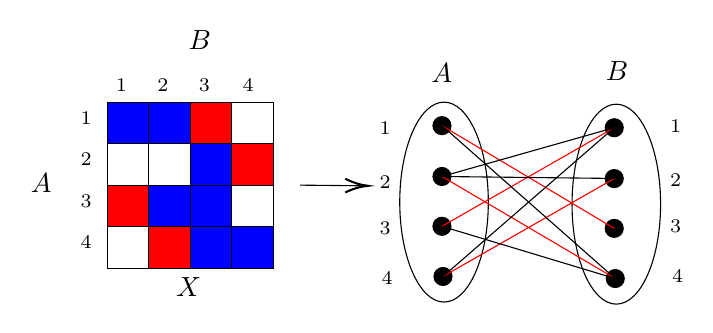
\begin{tikzpicture}[x=0.75pt,y=0.75pt,yscale=-1,xscale=1]
        %uncomment if require: \path (0,300); %set diagram left start at 0, and has height of 300

        %Shape: Grid [id:dp1111199869042343] 
        \draw  [draw opacity=0] (119,40) -- (199,40) -- (199,120) -- (119,120) -- cycle ; \draw   (139,40) -- (139,120)(159,40) -- (159,120)(179,40) -- (179,120) ; \draw   (119,60) -- (199,60)(119,80) -- (199,80)(119,100) -- (199,100) ; \draw   (119,40) -- (199,40) -- (199,120) -- (119,120) -- cycle ;
        %Shape: Rectangle [id:dp34703196177208884] 
        \draw  [fill={rgb, 255:red, 0; green, 0; blue, 255 }  ,fill opacity=1 ] (119,40) -- (139,40) -- (139,60) -- (119,60) -- cycle ;
        %Shape: Rectangle [id:dp6541634601571268] 
        \draw  [fill={rgb, 255:red, 0; green, 0; blue, 255 }  ,fill opacity=1 ] (139,40) -- (159,40) -- (159,60) -- (139,60) -- cycle ;
        %Shape: Rectangle [id:dp574711983476796] 
        \draw  [fill={rgb, 255:red, 0; green, 0; blue, 255 }  ,fill opacity=1 ] (159,60) -- (179,60) -- (179,80) -- (159,80) -- cycle ;
        %Shape: Rectangle [id:dp060811219131861494] 
        \draw  [fill={rgb, 255:red, 0; green, 0; blue, 255 }  ,fill opacity=1 ] (159,80) -- (179,80) -- (179,100) -- (159,100) -- cycle ;
        %Shape: Rectangle [id:dp16180262826121272] 
        \draw  [fill={rgb, 255:red, 0; green, 0; blue, 255 }  ,fill opacity=1 ] (139,80) -- (159,80) -- (159,100) -- (139,100) -- cycle ;
        %Shape: Rectangle [id:dp41023852521033766] 
        \draw  [fill={rgb, 255:red, 0; green, 0; blue, 255 }  ,fill opacity=1 ] (159,100) -- (179,100) -- (179,120) -- (159,120) -- cycle ;
        %Shape: Rectangle [id:dp63410711081005] 
        \draw  [fill={rgb, 255:red, 0; green, 0; blue, 255 }  ,fill opacity=1 ] (179,100) -- (199,100) -- (199,120) -- (179,120) -- cycle ;
        %Shape: Rectangle [id:dp8398838620439119] 
        \draw  [fill={rgb, 255:red, 255; green, 0; blue, 0 }  ,fill opacity=1 ] (159,40) -- (179,40) -- (179,60) -- (159,60) -- cycle ;
        %Shape: Rectangle [id:dp8159101832408716] 
        \draw  [fill={rgb, 255:red, 255; green, 0; blue, 0 }  ,fill opacity=1 ] (179,60) -- (199,60) -- (199,80) -- (179,80) -- cycle ;
        %Shape: Rectangle [id:dp41556757297740776] 
        \draw  [fill={rgb, 255:red, 255; green, 0; blue, 0 }  ,fill opacity=1 ] (119,80) -- (139,80) -- (139,100) -- (119,100) -- cycle ;
        %Shape: Rectangle [id:dp02623398340404892] 
        \draw  [fill={rgb, 255:red, 255; green, 0; blue, 0 }  ,fill opacity=1 ] (139,100) -- (159,100) -- (159,120) -- (139,120) -- cycle ;
        %Shape: Ellipse [id:dp2999064352294202] 
        \draw   (281.33,40) .. controls (293.12,40) and (302.67,61.56) .. (302.67,88.17) .. controls (302.67,114.77) and (293.12,136.33) .. (281.33,136.33) .. controls (269.55,136.33) and (260,114.77) .. (260,88.17) .. controls (260,61.56) and (269.55,40) .. (281.33,40) -- cycle ;
        %Straight Lines [id:da8678629117386351] 
        \draw    (212,80) -- (242.67,80.31) ;
        \draw [shift={(244.67,80.33)}, rotate = 180.58] [color={rgb, 255:red, 0; green, 0; blue, 0 }  ][line width=0.75]    (10.93,-3.29) .. controls (6.95,-1.4) and (3.31,-0.3) .. (0,0) .. controls (3.31,0.3) and (6.95,1.4) .. (10.93,3.29)   ;
        %Shape: Circle [id:dp5544933841591936] 
        \draw  [fill={rgb, 255:red, 0; green, 0; blue, 0 }  ,fill opacity=1 ] (276,51.33) .. controls (276,48.94) and (277.94,47) .. (280.33,47) .. controls (282.73,47) and (284.67,48.94) .. (284.67,51.33) .. controls (284.67,53.73) and (282.73,55.67) .. (280.33,55.67) .. controls (277.94,55.67) and (276,53.73) .. (276,51.33) -- cycle ;
        %Shape: Circle [id:dp6010843931346055] 
        \draw  [fill={rgb, 255:red, 0; green, 0; blue, 0 }  ,fill opacity=1 ] (276,75.83) .. controls (276,73.44) and (277.94,71.5) .. (280.33,71.5) .. controls (282.73,71.5) and (284.67,73.44) .. (284.67,75.83) .. controls (284.67,78.23) and (282.73,80.17) .. (280.33,80.17) .. controls (277.94,80.17) and (276,78.23) .. (276,75.83) -- cycle ;
        %Shape: Circle [id:dp34998711302514374] 
        \draw  [fill={rgb, 255:red, 0; green, 0; blue, 0 }  ,fill opacity=1 ] (276,99.83) .. controls (276,97.44) and (277.94,95.5) .. (280.33,95.5) .. controls (282.73,95.5) and (284.67,97.44) .. (284.67,99.83) .. controls (284.67,102.23) and (282.73,104.17) .. (280.33,104.17) .. controls (277.94,104.17) and (276,102.23) .. (276,99.83) -- cycle ;
        %Shape: Circle [id:dp7793138710668669] 
        \draw  [fill={rgb, 255:red, 0; green, 0; blue, 0 }  ,fill opacity=1 ] (276.5,124) .. controls (276.5,121.61) and (278.44,119.67) .. (280.83,119.67) .. controls (283.23,119.67) and (285.17,121.61) .. (285.17,124) .. controls (285.17,126.39) and (283.23,128.33) .. (280.83,128.33) .. controls (278.44,128.33) and (276.5,126.39) .. (276.5,124) -- cycle ;
        %Shape: Ellipse [id:dp979678000417449] 
        \draw   (364.33,41) .. controls (376.12,41) and (385.67,62.56) .. (385.67,89.17) .. controls (385.67,115.77) and (376.12,137.33) .. (364.33,137.33) .. controls (352.55,137.33) and (343,115.77) .. (343,89.17) .. controls (343,62.56) and (352.55,41) .. (364.33,41) -- cycle ;
        %Shape: Circle [id:dp33043017100090777] 
        \draw  [fill={rgb, 255:red, 0; green, 0; blue, 0 }  ,fill opacity=1 ] (359,52.33) .. controls (359,49.94) and (360.94,48) .. (363.33,48) .. controls (365.73,48) and (367.67,49.94) .. (367.67,52.33) .. controls (367.67,54.73) and (365.73,56.67) .. (363.33,56.67) .. controls (360.94,56.67) and (359,54.73) .. (359,52.33) -- cycle ;
        %Shape: Circle [id:dp024719195265869076] 
        \draw  [fill={rgb, 255:red, 0; green, 0; blue, 0 }  ,fill opacity=1 ] (359,76.83) .. controls (359,74.44) and (360.94,72.5) .. (363.33,72.5) .. controls (365.73,72.5) and (367.67,74.44) .. (367.67,76.83) .. controls (367.67,79.23) and (365.73,81.17) .. (363.33,81.17) .. controls (360.94,81.17) and (359,79.23) .. (359,76.83) -- cycle ;
        %Shape: Circle [id:dp5863778458097556] 
        \draw  [fill={rgb, 255:red, 0; green, 0; blue, 0 }  ,fill opacity=1 ] (359,100.83) .. controls (359,98.44) and (360.94,96.5) .. (363.33,96.5) .. controls (365.73,96.5) and (367.67,98.44) .. (367.67,100.83) .. controls (367.67,103.23) and (365.73,105.17) .. (363.33,105.17) .. controls (360.94,105.17) and (359,103.23) .. (359,100.83) -- cycle ;
        %Shape: Circle [id:dp9420168302156724] 
        \draw  [fill={rgb, 255:red, 0; green, 0; blue, 0 }  ,fill opacity=1 ] (359.5,125) .. controls (359.5,122.61) and (361.44,120.67) .. (363.83,120.67) .. controls (366.23,120.67) and (368.17,122.61) .. (368.17,125) .. controls (368.17,127.39) and (366.23,129.33) .. (363.83,129.33) .. controls (361.44,129.33) and (359.5,127.39) .. (359.5,125) -- cycle ;
        %Straight Lines [id:da36676573007002466] 
        \draw [color={rgb, 255:red, 255; green, 0; blue, 0 }  ,draw opacity=1 ]   (280.33,51.33) -- (363.33,100.83) ;
        %Straight Lines [id:da017289750597913267] 
        \draw [color={rgb, 255:red, 255; green, 0; blue, 0 }  ,draw opacity=1 ]   (280.33,75.83) -- (363.83,125) ;
        %Straight Lines [id:da6164540669805414] 
        \draw [color={rgb, 255:red, 255; green, 0; blue, 0 }  ,draw opacity=1 ]   (280.33,99.83) -- (363.33,52.33) ;
        %Straight Lines [id:da1330605140641683] 
        \draw [color={rgb, 255:red, 255; green, 0; blue, 0 }  ,draw opacity=1 ]   (280.83,124) -- (363.33,76.83) ;
        %Straight Lines [id:da01761054889840097] 
        \draw    (280.33,51.33) -- (363.83,125) ;
        %Straight Lines [id:da523567078096067] 
        \draw    (280.33,75.83) -- (363.33,52.33) ;
        %Straight Lines [id:da1866835538480368] 
        \draw    (280.33,75.83) -- (367.67,76.83) ;
        %Straight Lines [id:da6464527011200191] 
        \draw    (280.33,99.83) -- (363.83,125) ;
        %Straight Lines [id:da9038153780958647] 
        \draw    (280.83,124) -- (363.33,52.33) ;

        % Text Node
        \draw (151,123.4) node [anchor=north west][inner sep=0.75pt]    {$X$};
        % Text Node
        \draw (81,73.4) node [anchor=north west][inner sep=0.75pt]    {$A$};
        % Text Node
        \draw (157,4.4) node [anchor=north west][inner sep=0.75pt]    {$B$};
        % Text Node
        \draw (105,43.4) node [anchor=north west][inner sep=0.75pt]  [font=\scriptsize]  {$1$};
        % Text Node
        \draw (105,63.4) node [anchor=north west][inner sep=0.75pt]  [font=\scriptsize]  {$2$};
        % Text Node
        \draw (105,83.4) node [anchor=north west][inner sep=0.75pt]  [font=\scriptsize]  {$3$};
        % Text Node
        \draw (105,103.4) node [anchor=north west][inner sep=0.75pt]  [font=\scriptsize]  {$4$};
        % Text Node
        \draw (122,27.4) node [anchor=north west][inner sep=0.75pt]  [font=\scriptsize]  {$1$};
        % Text Node
        \draw (142,27.4) node [anchor=north west][inner sep=0.75pt]  [font=\scriptsize]  {$2$};
        % Text Node
        \draw (162,27.4) node [anchor=north west][inner sep=0.75pt]  [font=\scriptsize]  {$3$};
        % Text Node
        \draw (183,27.4) node [anchor=north west][inner sep=0.75pt]  [font=\scriptsize]  {$4$};
        % Text Node
        \draw (274,20.4) node [anchor=north west][inner sep=0.75pt]    {$A$};
        % Text Node
        \draw (249,48.4) node [anchor=north west][inner sep=0.75pt]  [font=\scriptsize]  {$1$};
        % Text Node
        \draw (249,74.4) node [anchor=north west][inner sep=0.75pt]  [font=\scriptsize]  {$2$};
        % Text Node
        \draw (249,96.4) node [anchor=north west][inner sep=0.75pt]  [font=\scriptsize]  {$3$};
        % Text Node
        \draw (250,120.4) node [anchor=north west][inner sep=0.75pt]  [font=\scriptsize]  {$4$};
        % Text Node
        \draw (389,47.4) node [anchor=north west][inner sep=0.75pt]  [font=\scriptsize]  {$1$};
        % Text Node
        \draw (389,73.4) node [anchor=north west][inner sep=0.75pt]  [font=\scriptsize]  {$2$};
        % Text Node
        \draw (389,95.4) node [anchor=north west][inner sep=0.75pt]  [font=\scriptsize]  {$3$};
        % Text Node
        \draw (390,119.4) node [anchor=north west][inner sep=0.75pt]  [font=\scriptsize]  {$4$};
        % Text Node
        \draw (358,19.4) node [anchor=north west][inner sep=0.75pt]    {$B$};
    \end{tikzpicture}
    \caption{Chess to Bipartition}
\end{figure}
Given a set $ X \subseteq A\times B $ of `allowable' squares in an $ A\times B $ array,
we can form a bipartite graph $ G(X) $ with partition $ (A,B) $
where $ a\in A $ is adjacent to $ b\in B $ if and only if the $ ab $-cell is in $ X $.
\begin{thmbox}
    \begin{prop}
        If $ |A|=|B|=n $, then we can place $ n $ non-attacking rooks in the array
        if and only if $ G $ has a perfect matching.
    \end{prop}
\end{thmbox}
By Hall's Theorem, there is a matching saturating $ A $ if and only if there
is no set $ A^\prime \subseteq A $ for which $ |N(A^\prime)|<|A^\prime| $.

If $ |N(A^\prime)|<|A^\prime| $ in $ G(X) $, then this means that every cell in $ A^\prime\times
    (B\setminus N(A^\prime)) $ is forbidden (not in $ X $).
But $ |A^\prime|+|B\setminus N(A^\prime)|= |A^\prime|+n-|N(A^\prime)|>n $.

\begin{thmbox}
    \begin{prop}
        Given a square $ A\times B $ array and a set $ F $ of forbidden squares
        $ (F\subseteq A\times B) $, either
        \begin{itemize}
            \item we can place $ n=|A|=|B| $ non-attacking rooks while avoiding all squares
                  in $ F $, or
            \item there is a set $ A^\prime\subseteq A $ and $ B^\prime\subseteq B $
                  such that $ |A^\prime|+|B^\prime|>n $ and every square in $ A^\prime\times B^\prime $
                  is forbidden.
        \end{itemize}
    \end{prop}
\end{thmbox}

\textbf{\underline{Linear Algebra}}
\[ \begin{pmatrix}
        \star & \star & 0     & 0     & \star & 0     & \star \\
        0     & 0     & \star & \star & 0     & \star & 0     \\
        0     & 0     & 0     & 0     & \star & 0     & \star \\
        0     & \star & \star & 0     & 0     & \star & 0     \\
        0     & \star & 0     & 0     & \star & 0     & 0     \\
        \star & 0     & 0     & 0     & \star & 0     & 0     \\
        0     & 0     & 0     & 0     & \star & 0     & \star
    \end{pmatrix}_{7\times 7}
\]
\underline{Question}: Given a square `$ \star $-$ 0 $-matrix' when can we find
non-zero entries for the $ \star $'s such that the matrix is non-singular.

Example: Row of $ 0 $'s forces singular.
\begin{thmbox}
    \begin{prop}
        Given a square `$ \star $-$ 0 $-matrix' with rows $ A $ and columns $ B $,
        either
        \begin{itemize}
            \item we can find non-zero entries for the $ \star $'s such that the determinant
                  is non-zero, or
            \item there is a set $ A^\prime\subseteq B $ and $ B^\prime \subseteq B $
                  such that $ |A^\prime|+|B^\prime|>n $ and every entries in $ A^\prime\times B^\prime $
                  is zero, so the determinant is forced to be $ 0 $.
        \end{itemize}
    \end{prop}
\end{thmbox}
\begin{proof}
    Apply Hall's Theorem.
\end{proof}

\underline{Sequel Courses}:
\begin{itemize}
    \item First half of MATH 239: CO 330 (Algebraic Enumeration)
    \item Second half of MATH 239: CO 342 (Graph Theory)
\end{itemize}
